\begin{inhalt}
\renewcommand*\chapterpagestyle{scrheadings}


\chapter{Hardwareentwicklung}

In diesem Kapitel geht es um die Entwicklung sowie den Aufbau der Hardware des Messgeräts. Dazu wurde eine Platine entworfen, um alle Komponenten miteinander zu verbinden und diese in ein dafür 3D-gedrucktes Gehäuse zu integrieren.
\smallskip
Das PCB wurde im 2-Layer-Design entworfen, da es für diese Anwendung ausreichend war.
Auf der Ober- und Unterseite des PCBs wurden jeweils Masseflächen angelegt, die mithilfe von Via-Stitching miteinander verbunden sind, um eine gute Verbindung herzustellen.
Die SMD-Bauteile befinden sich nur auf der Unterseite der Platine, um beidseitiges SMD-Löten zu vermeiden. Die SMD-Widerstände und die SMD-Kondensatoren sind im 1206-Format gewählt. Die Spule wurde im 3232-Format gewählt. Durch diese Größen lassen sich die erwähnten Komponenten auch per Hand mit dem Lötkolben leicht auflöten.
\newline
Als Leiterbahnbreite wurde 0,7mm gewählt. Der maximale Strom einer solchen Leitung entspricht …, was dem maximalen Strom des Gerätes (siehe …) leicht standhält.

\smallskip

\textbf{Gegebene Werte:}

\begin{align*}
\text{Leiterbahnbreite} &= 0{,}7\,\text{mm} = 27{,}56\,\text{mil} \\
\text{Kupferdicke} &= 35\,\mu\text{m} = 1{,}38\,\text{mil} \\
\text{Temperaturänderung } \Delta T &= 10\,^\circ\text{C}
\end{align*}



\vspace{1em}
\textbf{Querschnittsfläche:}

\begin{align*}
A &= \text{Breite} \times \text{Dicke} \\
A &= 27{,}56 \times 1{,}38 = 38{,}02\,\text{mil}^2
\end{align*}

\vspace{1em}
\textbf{Formel nach IPC-2221 (Außenlage):}

\begin{align*}
I &= 0{,}048 \cdot (\Delta T)^{0{,}44} \cdot A^{0{,}725} \\
I &= 0{,}048 \cdot (10)^{0{,}44} \cdot (38{,}02)^{0{,}725} \\
I &\approx 1{,}85\,\text{A}
\end{align*}

\section{Pin Zuordnungen}


   Um ein möglichst sauberes Design zu erreichen, wurde die Pin-Zuordnung des Mikrocontrollers folgendermaßen gewählt:

   \renewcommand{\arraystretch}{1.5}

\begin{table}[H]
\centering
\rowcolors{2}{white}{white}
\begin{tabular}{|l|c|}
\hline
\rowcolor{cyan!20}
\textbf{Pico W GPIO-Pin} & \textbf{Funktion} \\
\hline
GPIO0 & S1 \\
\hline
GPIO1 & S2 \\
\hline
GPIO4 & SDA \\
\hline
GPIO5 & SCL \\
\hline
GPIO6 & Busy \\
\hline
GPIO7 & RST \\
\hline
GPIO8 & DC \\
\hline
GPIO9 & CS \\
\hline
GPIO10 & CLK \\
\hline
GPIO11 & DIN (MOSI) \\
\hline
\end{tabular}
\caption{GPIO-Zuordnung des Pico W}
\label{tab:GPIO_Zuordnung}
\end{table}

In Tabelle \ref{tab:GPIO_Zuordnung} entsprechen S1 und S2 den beiden Tastern. 


      \section{USB-C}

      Das Messgerät benutzt USB-C für die Spannungsversorgung. Da nur die Versorgungsleitungen des USB-Busses benutzt werden, wird eine USB4125-Buchse verwendet (Kap. \ref{sec:USB4125_75}). Diese hat nur die Versorgungs-, GND- und CC-Pins, welche ausreichend sind, da keine Daten übertragen werden müssen. Ebenfalls erleichtert diese Buchse das Auflöten auf die Platine.

\begin{figure}[!htb]
\centering
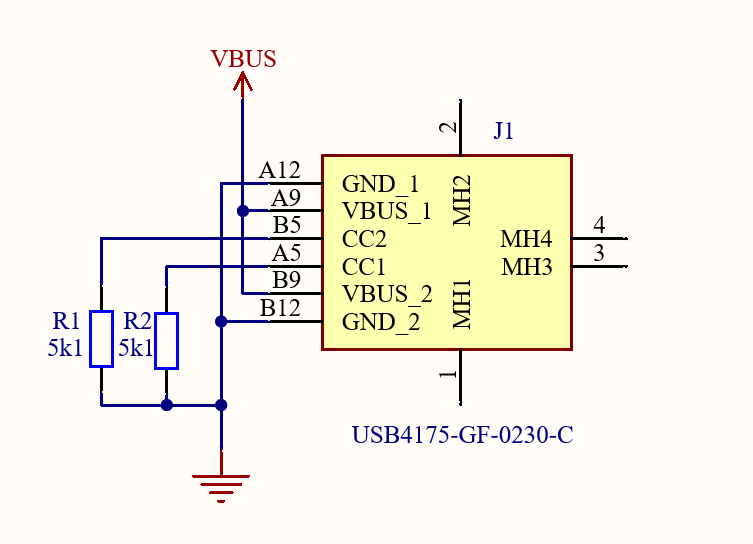
\includegraphics[width=0.75\textwidth]{files/Tobias/pics/Schaltungen/Schematik/USBC_Schematik.PNG}
\caption[USB-C Schematik]{USB-C Schematik}
\label{fig:USB-C_Schematik}
\end{figure}

Wie in Abbildung \ref{fig:USB-C_Schematik} zu sehen ist, sind beide CC-Pins der USB-C-Buchse über 5,1-k$\Omega$ Widerstände mit GND verbunden. Bei USB-C erfolgt über diese Pins der Austausch über die Verbindungskonfigurationen. Die 5,1-k$\Omega$ Widerstände signalisieren, dass es sich bei dem angeschlossenen Gerät um einen Verbraucher handelt, der maximal 15W Leistung aufnehmen darf \cite{USBC_Kommunikation}.

\begin{figure}[H] 
  \centering

  \begin{subfigure}[b]{0.48\textwidth}
    \centering
    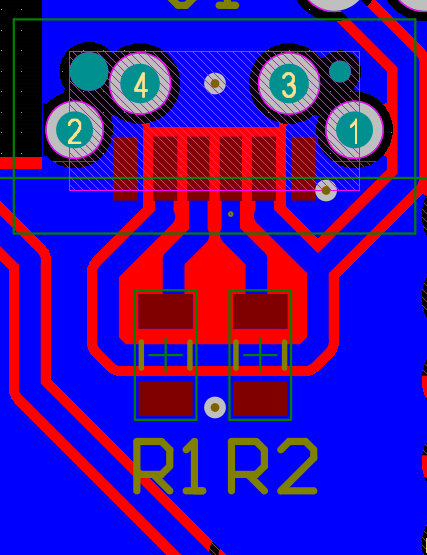
\includegraphics[height=7cm]{files/Tobias/pics/Schaltungen/PCB/USB_C_PCB.PNG}
    \caption{USB-C Bottom Layer}
    \label{fig:USB-C_Bottom_layer}
  \end{subfigure}
  \hfill
  \begin{subfigure}[b]{0.48\textwidth}
    \centering
    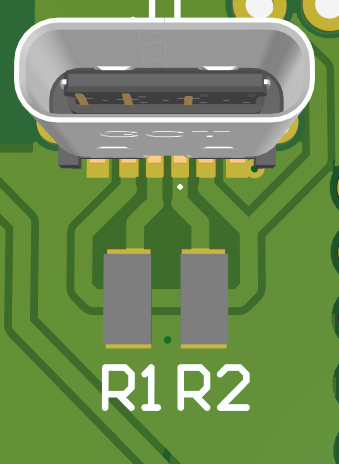
\includegraphics[height=7cm]{files/Tobias/pics/Schaltungen/PCB/USB_C_PCB_3D.PNG}
    \caption{USB-C 3D Ansicht}
    \label{fig:USB-C_3D_Ansicht}
  \end{subfigure}

  \caption{USB-C PCB Ansicht}
  \label{fig:pcb_layers}
\end{figure}



      \section{3,3V Spannungsregler}

Da der Mikrocontroller, die Sensoren sowie das Display mit 3,3V arbeiten und die USB-C-Versorgung 5V bereitstellt, ist ein Spannungsregler notwendig. Verwendet wird der NJM12856 \cite{NJM12856}, da dieser mit 1000mA dem maximalen Strom des Geräts standhält (Tab. \ref{tab:Stromverbrauch}).

Um den maximalen Stromverbrauch des Gerätes zu bestimmen, wurden folgende Werte aus den Datenblättern der einzelnen Komponenten entnommen: 


\renewcommand{\arraystretch}{1.5}

\begin{table}[H]
\centering
\rowcolors{2}{white}{white}
\begin{tabular}{|l|c|}
\hline
\rowcolor{cyan!20}
\textbf{Komponente} & \textbf{max. Stromaufnahme} \\
\hline
BME688 & 18\,mA \\
\hline
PAS CO\textsubscript{2} & 160\,mA \\
\hline
Display & 45\,mA \\
\hline
Raspberry Pi Pico W & 300\,mA \\
\hline
\end{tabular}
\caption{max. Stromverbrauch der Hauptkomponenten}
\label{tab:Stromverbrauch}
\end{table}

Da für den Raspberry Pico W keine genaue Angabe über den Stromverbrauch im Datenblatt zu finden ist, wurde der obige Wert durch Internetrecherche \cite{PicoWCurrent} und unter Einbezug der benutzten Bussysteme sowie der WLAN-Verbindung geschätzt.

\begin{figure}[!htb]
\centering
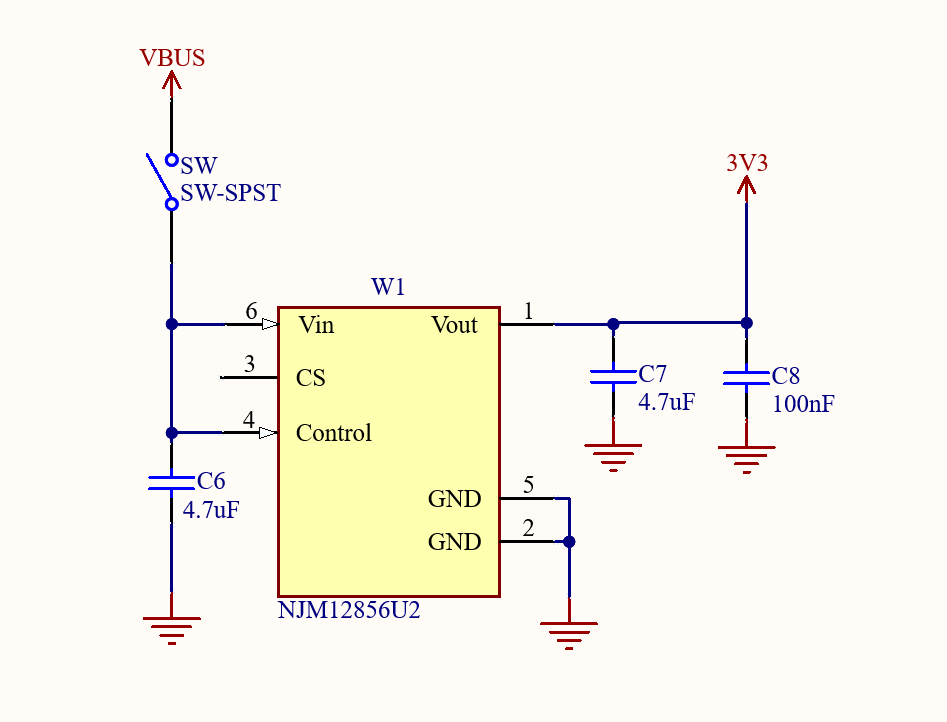
\includegraphics[width=0.75\textwidth]{files/Tobias/pics/Schaltungen/Schematik/3V3_Converter_Schematik.PNG}
\caption[3,3V Spannungsregler Schematik]{3,3V Spannungsregler Schematik}
\label{fig:3,3V Spannungsregler Schematik}
\end{figure}

Wie in Abbildung \ref{fig:3,3V Spannungsregler Schematik} zu sehen ist, wurde am Ein- und Ausgang des NJM12856 jeweils ein 4,7µF-Kondensator hinzugefügt, um stabile Spannungen zu gewährleisten. Zusätzlich wurde ein weiterer 100nF-Kondensator am Ausgang des NJM12856 hinzugefügt, um mögliche Störungen zu minimieren. Der CS-Pin bleibt offen, da kein Softstart benötigt wird \cite{NJM12856}. 2 Pins wurden für einen Schalter inkludiert, um die gesamte Spannungsversorgung vom Gerät zu trennen. 


\begin{figure}[H] 
  \centering

  \begin{subfigure}[b]{0.48\textwidth}
    \centering
    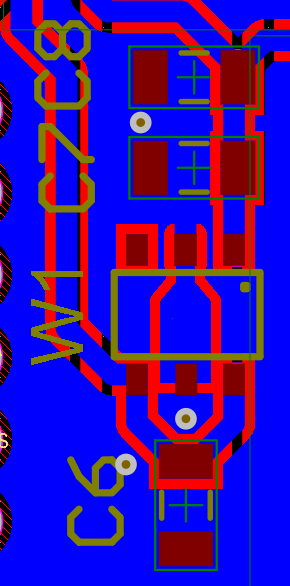
\includegraphics[height=7cm]{files/Tobias/pics/Schaltungen/PCB/3V3_Spannungregler_PCB.PNG}
    \caption{3,3V Spannungsregler Bottom Layer}
    \label{fig:USB-C_Bottom_layer}
  \end{subfigure}
  \hspace{2mm} % <-- Abstand verkleinert
  \begin{subfigure}[b]{0.48\textwidth}
    \centering
    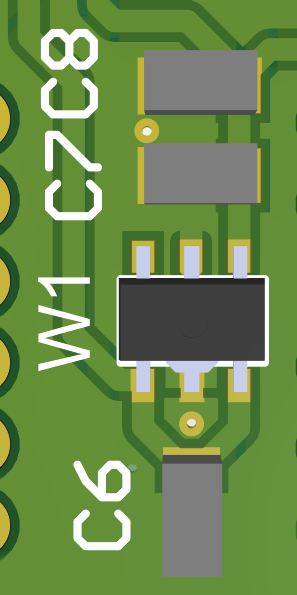
\includegraphics[height=7cm]{files/Tobias/pics/Schaltungen/PCB/3V3_Spannungsregler_PCB_3D.PNG}
    \caption{3,3V Spannungsregler 3D Ansicht}
    \label{fig:USB-C_3D_Ansicht}
  \end{subfigure}

  \caption{3,3V Spannungsregler PCB Ansicht}
  \label{fig:pcb_layers}
\end{figure}








      \section{12V Spannungwandler}
      
Der PASCO2V01-Sensor benötigt neben der 3,3V-Spannungsversorgung ebenfalls eine 12V-Spannungsversorgung. Der Aufwärtswandler TLV61046ADBVR \cite{TLV61046} wird dafür benutzt. Dieser ist in dem Datenblatt für Design-Richtlinien des PASCO2V01 \cite{PASCO2_Design_Guidelines}, inklusive Beschaltung, empfohlen.


\begin{figure}[!htb]
\centering
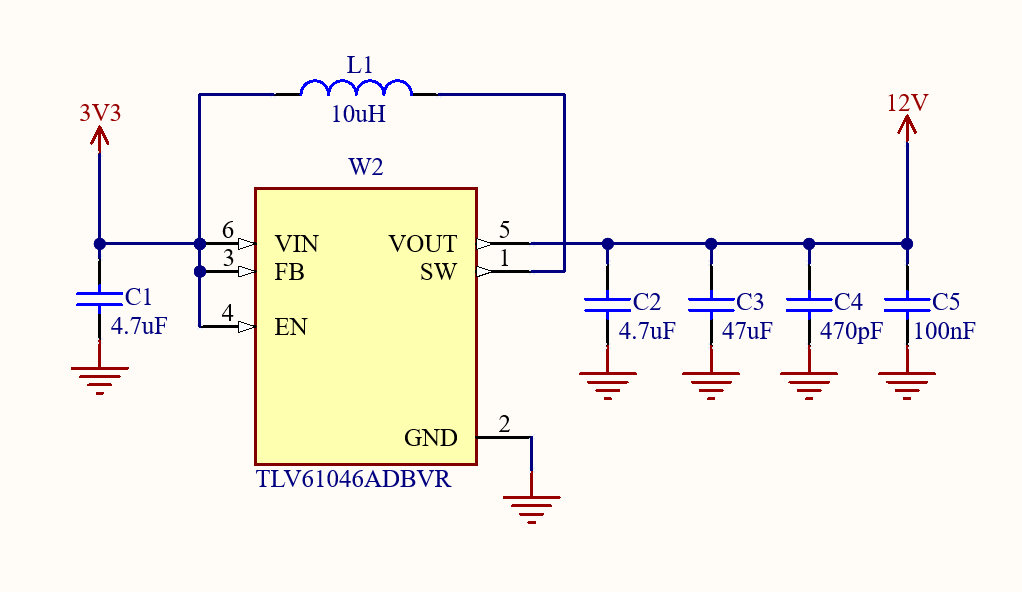
\includegraphics[width=0.75\textwidth]{files/Tobias/pics/Schaltungen/Schematik/12V_Converter_Schematik.PNG}
\caption[12V Spannungswandler Schematik]{12V Spannungswandler Schematik}
\label{fig:12V Spannungswandler Schematik}
\end{figure}

Die Beschaltung des TLV61046ADBVR (Abb. \ref{fig:12V Spannungswandler Schematik}) wurde entsprechend dem Datenblatt für Design-Richtlinien des PASCO2V01 \cite{PASCO2_Design_Guidelines} entnommen. 


\begin{figure}[H] 
  \centering

  \begin{subfigure}[b]{0.48\textwidth}
    \centering
    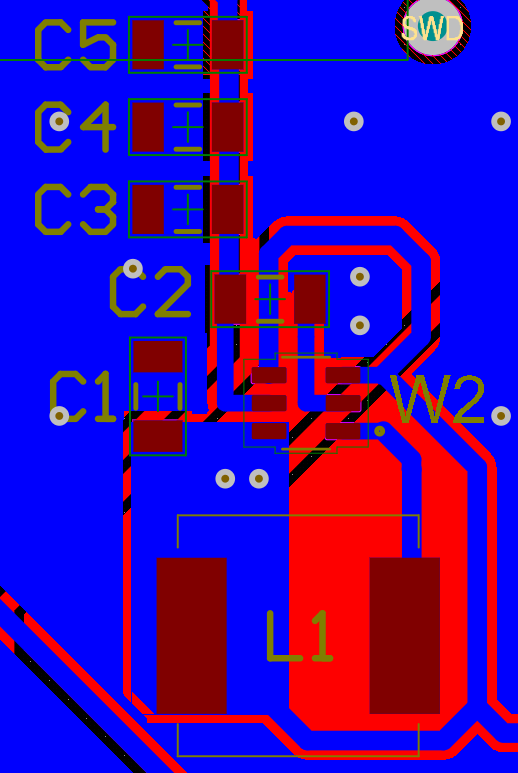
\includegraphics[height=7cm]{files/Tobias/pics/Schaltungen/PCB/12V_Spannungswandler_PCB_.PNG}
    \caption{12V Spannungswandler Bottom Layer}
    \label{fig:12V_Bottom_layer}
  \end{subfigure}
  \hfill
  \begin{subfigure}[b]{0.48\textwidth}
    \centering
    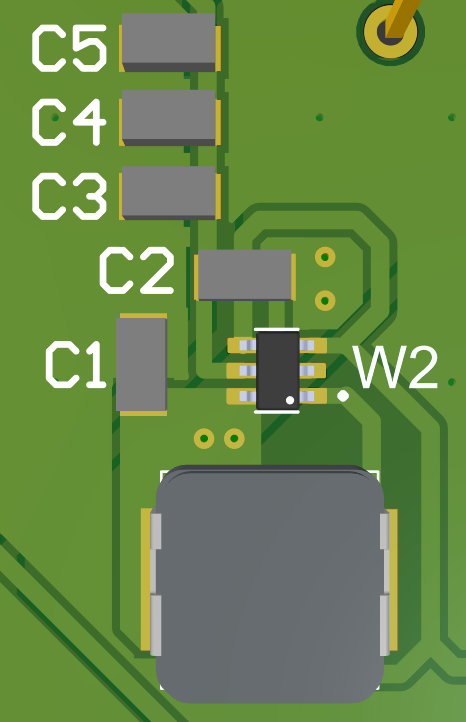
\includegraphics[height=7cm]{files/Tobias/pics/Schaltungen/PCB/12V_Spannungswandler_PCB_3D.PNG}
    \caption{12V Spannungswandler 3D Ansicht}
    \label{fig:12V_3D_Ansicht}
  \end{subfigure}

  \caption{12V Spannungswandler PCB Ansicht}
  \label{fig:pcb_layers}
\end{figure}
      

   \section{Mikrocontroller}


   

   \section{PCB Version 1}
   \label{ref:PCB_Version_1}
   \section{PCB Version 2}

\section{Fertigung des PCBs/Prints}

\section{Messungen}
	\subsection{Spannungen}
	\subsection{I2C}
	\subsection{SPI}

\end{inhalt}